% fig06_pic_parity.tex — 1-D linear PIC parity: FBPIC-measured plasma
% wavelength vs the cold-linear closed form at n_e=1e18 cm^-3. A zoomed
% y-axis (31.5-34) makes the Delta=3.56% gap visible; the closed-form
% reference is the dashed line. Compiled to PDF for Appendix C.
%
% Data: verify-ledger.json plasma_wakefield_pic_parity + the
% pic_parity_1e18() pins in plasma_wakefield.hexa (PR #1088).
%   closed-form lambda_p = 33.38943 um   (Dawson, Appendix B)
%   FBPIC 0.27.0 (a0=0.1)  = 32.20017 um  -> Delta = 3.562%
% Grid Nz=512 Nr=40 Nm=2, 1792 steps, on-axis Ez zero-crossing period.
%
% Manual single-shot compile (debug):
%   xelatex -interaction=nonstopmode -halt-on-error fig06_pic_parity.tex
\documentclass[border=4pt]{standalone}
\usepackage{tikz}
\usepackage{pgfplots}
\pgfplotsset{compat=1.18}
\begin{document}
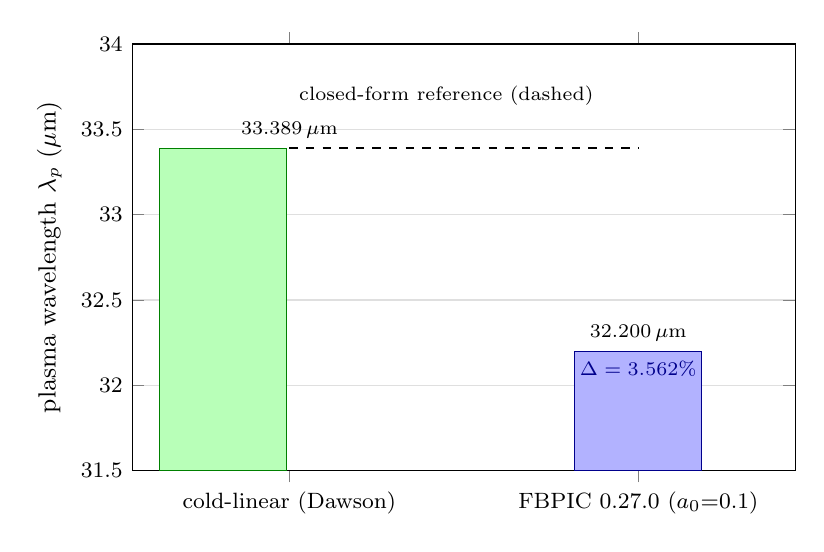
\begin{tikzpicture}
\begin{axis}[
  width=10cm, height=7cm,
  ybar,
  bar width=46pt,
  ymin=31.5, ymax=34.0,
  ylabel={plasma wavelength $\lambda_p$ ($\mu$m)},
  symbolic x coords={closed-form, FBPIC},
  xtick={closed-form, FBPIC},
  xticklabels={cold-linear (Dawson), FBPIC 0.27.0 ($a_0{=}0.1$)},
  x tick label style={font=\footnotesize},
  tick label style={font=\footnotesize},
  label style={font=\small},
  ymajorgrids,
  grid style={gray!25},
  enlarge x limits=0.45,
  /pgf/number format/.cd, fixed, precision=3,
]
% closed-form reference dashed line
\addplot[draw=black,dashed,thick,sharp plot,update limits=false] coordinates {
  (closed-form,33.38943) (FBPIC,33.38943)
};
\addplot[draw=green!50!black,fill=green!28] coordinates {(closed-form,33.38943)};
\addplot+[draw=blue!55!black,fill=blue!30,bar shift=0pt] coordinates {(FBPIC,32.20017)};
% annotations
\node[font=\scriptsize,anchor=south] at (axis cs:closed-form,33.38943) {33.389\,$\mu$m};
\node[font=\scriptsize,anchor=south] at (axis cs:FBPIC,32.20017) {32.200\,$\mu$m};
\node[font=\scriptsize,anchor=north,text=blue!55!black] at (axis cs:FBPIC,32.20017)
  {$\Delta = 3.562\%$};
\node[font=\scriptsize,text=black,anchor=west] at (axis cs:closed-form,33.7)
  {closed-form reference (dashed)};
\end{axis}
\end{tikzpicture}
\end{document}
